\newcommand{\model}{%
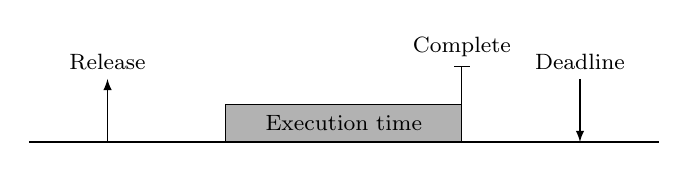
\begin{tikzpicture}[
  yscale = 0.8,
  normal/.style={fill=black!30},
  release/.style={-latex},
  complet/.style={-|},
  every text node part/.style={align=center}
]
%general params
\def\th{.6} %task height
\def\blockdim{(.4,.4)}
\def\arrowdim{(0,.5)}
\def\arrowdimB{(0,.4)}

%axes
\draw[thick, black] (0,0) -- (8, 0);

%L1
\draw[release] (1, 0) -- +(0,1) node[above] {{\footnotesize Release}};
\draw[normal]  (2.5, 0) rectangle +(3, \th) node[midway] {{\footnotesize Execution time}};
\draw[complet] (5.5, 0) -- +(0, 1.2) node[above] {{\footnotesize Complete}};
\draw[release] (7, 1) node[above] {{\footnotesize Deadline}} -- (7,0);

\end{tikzpicture}
}

\newcommand{\smallqueue}[2]{%
\draw[queuesty] (#1)node[right,xshift=.1cm]{\sffamily #2}-- ++(.2,.15)-- ++(.8,0)-- ++(0,-.3)-- ++(-.8,0)-- cycle;}
\newcommand{\bigqueue}[2]{%
\draw[queuesty] (#1)node[right,xshift=.2cm]{\sffamily #2}-- ++(.3,.3)-- ++(.8,0)-- ++(0,-.6)-- ++(-.8,0)-- cycle;}

\newcommand{\MrsP}[2]{%
\begin{tikzpicture}[
  xscale=#1,
  yscale=#2,
  every node/.append style={transform shape},
  queuesty/.style={fill=white, very thick, font=\tiny},
  cpusty/.style={fill=gray!40, draw, circle, minimum width=1cm},
  srpsty/.style={fill=white, draw, circle, text width=.17cm, font=\tiny, very thick},
  ressty/.style={fill=red!30, draw, very thick, rounded corners=5pt},
  arrow/.style={->,>=stealth},
  littletext/.style={font=\sffamily\tiny,inner sep=0pt,outer sep=-2pt,fill=white},
  emptytask/.style={rectangle, minimum width=.7cm,font=\footnotesize},
  taskA/.style={fill=green!40, draw, rectangle, minimum width=.7cm,font=\footnotesize},
  taskB/.style={fill=orange!40!yellow, draw, rectangle, minimum width=.7cm,font=\footnotesize}]

\begin{scope}[xshift=4cm, yshift=1cm]
\coordinate (SRP1node) at (0,0);
\node[cpusty] (P1) at (2.5,0) {$P_1$};
\node[taskA] (T1) at (1.3,.4) {$\tau_1$};
\node[emptytask]  at (1.3,0) {$\cdots$};
\node[taskA] (Tx) at (1.3,-.4) {$\tau_x$};
\draw[arrow] (T1.east) -- (P1.west);
\draw[arrow] (Tx.east) -- (P1.west);
\draw[dashed, thin] ([shift={(-.1,.2)}]T1.north-|SRP1node) node[right,xshift=.3cm,littletext]{partition$_1$} rectangle ([shift={(.1,-.1)}]Tx.south-|P1.east);
\node[srpsty] (SRP1) at (SRP1node) {}; \node[font=\sffamily\tiny] at(SRP1node.east){SRP};
\draw[arrow] (T1.west) to[out=180,in=0] ([yshift=.1cm]SRP1.east);
\draw[arrow] (Tx.west) to[out=180,in=0] ([yshift=-.1cm]SRP1.east);
\end{scope}
\node[emptytask] at (5,0) {$\cdots$};
\begin{scope}[xshift=4cm, yshift=-1.1cm]
\coordinate (SRPmnode) at (0,0);
\node[cpusty] (Pm) at (2.5,0) {\!$P_m$};
\node[taskB] (Ty) at (1.3,.4) {$\tau_y$};
\node[emptytask]  at (1.3,0) {$\cdots$};
\node[taskB] (Tn) at (1.3,-.4) {$\tau_n$};
\draw[arrow] (Ty.east) -- (Pm.west);
\draw[arrow] (Tn.east) -- (Pm.west);
\draw[dashed, thin] ([shift={(-.1,.2)}]Ty.north-|SRPmnode) node[right,xshift=.3cm,littletext]{partition$_m$} rectangle ([shift={(.1,-.1)}]Tn.south-|Pm.east);
\node[srpsty] (SRPm) at (SRPmnode) {}; \node[font=\sffamily\tiny] at(SRPmnode.east){SRP};
\draw[arrow] (Ty.west) to[out=180,in=0] ([yshift=.1cm]SRPm.east);
\draw[arrow] (Tn.west) to[out=180,in=0] ([yshift=-.1cm]SRPm.east);

\end{scope}

\begin{scope}
\draw[ressty] (0,-.25) rectangle +(1.5,.5) node[midway]{res$_k$};
\smallqueue{1.3,0}{FIFO}
\draw[|-|] (1.5, .35) -- ++(.8,0)node[midway,fill=white,font=\tiny]{$m$};
\end{scope}

\draw[arrow] (SRP1.west)node[anchor=south east,yshift=-.2cm,,font=\tiny\sffamily]{ \begin{tabular}{c} spinning at\\own ceiling\end{tabular}} to[out=180,in=0] (2.3,.1);
\draw[arrow] (SRPm.west)node[anchor=north east,yshift=.2cm,font=\tiny\sffamily]{ \begin{tabular}{c} spinning at\\own ceiling\end{tabular}} to[out=180,in=0] (2.3,-.1);

\end{tikzpicture}}

\newcommand{\OMIP}[2]{%
\begin{tikzpicture}[
  xscale=#1,
  yscale=#2,
  every node/.append style={transform shape},
  queuesty/.style={fill=white, very thick, font=\tiny},
  cpusty/.style={fill=gray!40, draw, circle, text width=.4cm,font=\scriptsize},
  srpsty/.style={fill=white, draw, circle, text width=.17cm, font=\tiny, very thick},
  ressty/.style={fill=red!30, draw, very thick, rounded corners=5pt},
  arrow/.style={->,>=stealth},
  littletext/.style={font=\sffamily\tiny,inner sep=0pt,outer sep=-2pt,fill=white},
  emptytask/.style={rectangle, minimum width=.7cm,font=\footnotesize},
  taskA/.style={fill=green!40, draw, rectangle, minimum width=.7cm,font=\footnotesize},
  taskB/.style={fill=orange!40!yellow, draw, rectangle, minimum width=.7cm,font=\footnotesize}]

\begin{scope}
\draw[ressty] (0,-.25) rectangle +(1.5,.5) node[midway]{res$_k$};
\smallqueue{1.3,0}{FIFO}
\draw[|-|] (1.5, .35) -- ++(.8,0)node[midway,fill=white,font=\tiny]{\textcolor{red}{$v$}};
\end{scope}


\begin{scope}
\node[taskA] (T1)  at(6.3,2.0) {$\tau_1$};
\node[emptytask]   at(6.3,1.5) {$\cdots$};
\node[taskA] (Tx)  at(6.3,1.0) {$\tau_x$};
\node[cpusty] (P1) at(8.0,2.2) {\!$P_{1,\textcolor{blue}{1}}$};
\node[emptytask]   at(8.0,1.5) {$\cdots$};
\node[cpusty] (Pc) at(8.0,0.8) {\!\!$P_{1,\textcolor{blue}{c}}$};
\draw[arrow] (T1.west) to[out=180,in=0] (5.2,1.6);
\draw[arrow] (Tx.west) to[out=180,in=0] (5.2,1.4);
\draw[arrow] (T1.east) -- (7.25, 1.5) -- (P1.south west);
\draw[arrow] (Tx.east) -- (7.25, 1.5) -- (Pc.north west);
\draw[fill=gray] (7.25,1.5) circle (.1) node(G1){};
\draw[dashed, thin] ([shift={(-2.6cm,+.1cm)}]P1.north-|T1.west)node[right,xshift=.3cm,littletext]{cluster\textcolor{red}{$_1$}} rectangle ([shift={(.2,-.2)}]Pc.south east);
\draw[|-|] (3.5,1.85) -- ++(.8,0)node[midway,fill=white,font=\tiny]{\textcolor{blue}{$c$}};
\smallqueue{3.3,1.5}{FIFO}
\bigqueue{4.1,1.5}{PRIO}
\node[rotate=90,anchor=north,littletext] at(5.6,1.5){suspend};
\end{scope}

\begin{scope}
\node[taskB] (Ty)  at(6.3,-1.0) {$\tau_y$};
\node[emptytask]   at(6.3,-1.5) {$\cdots$};
\node[taskB] (Tn)  at(6.3,-2.0) {$\tau_n$};
\node[cpusty] (Pcm) at(8.0,-0.8) {\!$P_{v,\textcolor{blue}{1}}$};
\node[emptytask]   at(8.0,-1.5) {$\cdots$};
\node[cpusty] (Pm) at(8.0,-2.2) {\!\!$P_{v,\textcolor{blue}{c}}$};
\draw[arrow] (Ty.west) to[out=180,in=0] (5.2,-1.4);
\draw[arrow] (Tn.west)  to[out=180,in=0] (5.2,-1.6);
\draw[arrow] (Ty.east) -- (7.25, -1.5) -- (Pcm.south west);
\draw[arrow] (Tn.east) -- (7.25, -1.5) -- (Pm.north west);
\draw[fill=gray] (7.25,-1.5) circle (.1) node(G2){};
\draw[dashed, thin] ([shift={(-2.6cm,+.1cm)}]Pcm.north-|Ty.west)node[right,xshift=.3cm,littletext]{cluster\textcolor{red}{$_v$}} rectangle ([shift={(.2,-.2)}]Pm.south east);
\draw[|-|] (3.5,-1.15) -- ++(.8,0)node[midway,fill=white,font=\tiny]{\textcolor{blue}{$c$}};
\smallqueue{3.3,-1.5}{FIFO}
\bigqueue{4.1,-1.5}{PRIO}
\node[rotate=90,anchor=north,littletext] at(5.6,-1.5){suspend};
\end{scope}

\draw[arrow] (3.3,1.5)node[anchor=south east,font=\tiny\sffamily]{copy head} to[out=180,in=0] (2.3,0.1);
\draw[arrow] (3.3,-1.5)node[anchor=north east,font=\tiny\sffamily]{copy head} to[out=180,in=0] (2.3,-0.1);

\node[xshift=-.1,font=\tiny\sffamily](JLFP) at(7.25,0){\textcolor{black!75}{JLFP scheduler}};
\draw[dotted,thin] (G1.center) -- (JLFP.center);
\draw[dotted,thin] (G2.center) -- (JLFP.center);

\end{tikzpicture}}

\newcommand{\MigrationMrsP}[2]{%
\begin{tikzpicture}[
  xscale=#1,
  yscale=#2,
  normal/.style={ fill=black!30},
  resource/.style={ fill=black!80},
  spinning/.style={fill=white, postaction={pattern=horizontal lines}},
  blocked/.style={fill=black!10, postaction={pattern=north east lines, very thin}},
  invprio/.style={fill=black!10, postaction={pattern=crosshatch, very thin}},
  release/.style={-latex},
  request/.style={-o},
  complet/.style={-|}]
%general params
\def\th{.4}
\def\tay{0}
\def\tby{1}
\def\tcy{3}
\def\tdy{4}
\def\blockdim{(.4,.4)}
\def\arrowdim{(0,.5)}
\def\arrowdimB{(0,.4)}
\coordinate (legend) at (1,6);
%tasklines
\draw[very thin, gray] (-.7,\tay)node[above,left,black]{$\tau_1$} -- +(15.2,0);
\draw[very thin, gray] (-.7,\tby)node[above,left,black]{$\tau_2$} -- +(15.2,0);
\node[left,font=\footnotesize] at(-1.8, .5) {$P_1$};
%\draw [decorate,decoration={brace,amplitude=10pt},xshift=-4pt,yshift=0pt] (-1.7,-0.5) -- (-1.7,1.5) node [black,midway,xshift=-0.6cm] {$P_1$};
\draw[very thin, gray] (-.7,\tcy)node[above,left,black]{$\tau_3$} -- +(15.2,0);
\draw[very thin, gray] (-.7,\tdy)node[above,left,black]{$\tau_4$} -- +(15.2,0);
\node[left,font=\footnotesize] at(-1.8, 3.5) {$P_2$};
%\draw [decorate,decoration={brace,amplitude=10pt},xshift=-4pt,yshift=0pt] (-1.7,2.5) -- (-1.7,4.5) node [black,midway,xshift=-0.6cm] {$P_2$};
%axes
\draw[thick, black, ->] (-.5,-1) -- (-.5, 5.3) node[rotate=90, left, above]{{\footnotesize prio}};
\draw[thick, black, ->] (-1,-.5) -- (15, -.5) node[below] {{\footnotesize time}};
\foreach \x in {0,...,14}\draw[thin, black] (\x, -.6)node[below]{\tiny $\x$} -- (\x, -.4);

%Task1
\draw[normal] (0, \tay) rectangle +(1, \th);
\draw[normal] (9, \tay) rectangle +(2, \th);
%Task2
\draw[normal] (1, \tby) rectangle +(2, \th);
\fill[spinning] (3, \tby) rectangle +(1, \th);
\draw[resource] (6, \tby) rectangle +(2, \th);
\draw[normal] (8, \tby) rectangle +(1, \th);
%Task3
\draw[normal] (0, \tcy) rectangle +(2, \th);
\draw[resource] (2, \tcy) rectangle +(4, \th);
\draw[normal] (7, \tcy) rectangle +(2, \th);
%Task4
\draw[normal] (4, \tdy) rectangle +(3, \th);

%Events
\draw[release] (0,\tay) -- +(0, .8);
\draw[release] (1,\tby) -- +(0, .8);
\draw[release] (0,\tcy) -- +(0, .8);
\draw[release] (4,\tdy) -- +(0, .8);
\draw[request] (3,\tby) -- +(0, .8);
\draw[request] (2,\tcy) -- +(0, .8);
\draw[complet] (11,\tay) -- +(0, .7);
\draw[complet] (9,\tby) -- +(0, .7);
\draw[complet] (9,\tcy) -- +(0, .7);
\draw[complet] (7,\tdy) -- +(0, .7);

\draw[thick, red, dashed] (-3,2.3) -- (4,2.3) -- ++(0, 1.5) -- ++(2, 0) -- ++(0,-1.5) -- (16, 2.3);

%Legend
%\draw[normal]   ($( 0.0,0.0) + (legend)$) node[below]{\tiny executing}          rectangle +\blockdim;
%\draw[resource] ($( 2.5,0.0) + (legend)$) node[below]{\tiny holding res.}       rectangle +\blockdim;
%\fill[spinning] ($( 5.0,0.0) + (legend)$) node[below]{\tiny busy wait} rectangle +\blockdim;
%\draw[release]  ($( 7.5,0.0) + (legend)$) node[below]{\tiny release}        -- +\arrowdim;
%\draw[request]  ($(10.0,0.0) + (legend)$) node[below]{\tiny request res.}       -- +\arrowdim;
%\draw[complet]  ($(12.5,0.0) + (legend)$) node[below]{\tiny completion}     -- +\arrowdimB;

\end{tikzpicture}}

\newcommand{\MigrationOMIP}[2]{%
\begin{tikzpicture}[
  xscale=#1,
  yscale=#2,
  normal/.style={ fill=black!30},
  resource/.style={ fill=black!80},
  spinning/.style={fill=white, postaction={pattern=horizontal lines}},
  blocked/.style={fill=black!10, postaction={pattern=north east lines, very thin}},
  invprio/.style={fill=black!10, postaction={pattern=crosshatch, very thin}},
  release/.style={-latex},
  request/.style={-o},
  complet/.style={-|}]
%general params
\def\th{.4}
\def\tay{0}
\def\tby{1}
\def\tcy{3}
\def\tdy{4}
\def\blockdim{(.4,.4)}
\def\arrowdim{(0,.5)}
\def\arrowdimB{(0,.4)}
\coordinate (legend) at (1,6);
%tasklines
\draw[very thin, gray] (-.7,\tay)node[above,left,black]{$\tau_1$} -- +(15.2,0);
\draw[very thin, gray] (-.7,\tby)node[above,left,black]{$\tau_2$} -- +(15.2,0);
\node[left,font=\footnotesize] at(-1.5, .5) {$\text{cluster}_1$};
%\draw [decorate,decoration={brace,amplitude=10pt},xshift=-4pt,yshift=0pt] (-1.7,-0.5) -- (-1.7,1.5) node [black,midway,xshift=-0.6cm] {\footnotesize$\text{cluster}_1$};
\draw[very thin, gray] (-.7,\tcy)node[above,left,black]{$\tau_3$} -- +(15.2,0);
\draw[very thin, gray] (-.7,\tdy)node[above,left,black]{$\tau_4$} -- +(15.2,0);
\node[left,font=\footnotesize] at(-1.5, 3.5) {$\text{cluster}_2$};
%\draw [decorate,decoration={brace,amplitude=10pt},xshift=-4pt,yshift=0pt] (-1.7,2.5) -- (-1.7,4.5) node [black,midway,xshift=-0.6cm] {\footnotesize$\text{cluster}_2$};
%axes
\draw[thick, black, ->] (-.5,-1) -- (-.5, 5.3) node[rotate=90, left, above]{{\footnotesize prio}};
\draw[thick, black, ->] (-1,-.5) -- (15, -.5) node[below] {{\footnotesize time}};
\foreach \x in {0,...,14}\draw[thin, black] (\x, -.6)node[below]{\tiny $\x$} -- (\x, -.4);

%Task1
\draw[normal] (0, \tay) rectangle +(1, \th);
\draw[normal] (3, \tay) rectangle +(1, \th);
\draw[normal] (9, \tay) rectangle +(1, \th);
%Task2
\draw[normal] (1, \tby) rectangle +(2, \th);
\draw[resource] (6, \tby) rectangle +(2, \th);
\draw[normal] (8, \tby) rectangle +(1, \th);
%Task3
\draw[normal] (0, \tcy) rectangle +(2, \th);
\draw[resource] (2, \tcy) rectangle +(4, \th);
\draw[normal] (7, \tcy) rectangle +(2, \th);
%Task4
\draw[normal] (4, \tdy) rectangle +(3, \th);

%Events
\draw[release] (0,\tay) -- +(0, .8);
\draw[release] (1,\tby) -- +(0, .8);
\draw[release] (0,\tcy) -- +(0, .8);
\draw[release] (4,\tdy) -- +(0, .8);
\draw[request] (3,\tby) -- +(0, .8);
\draw[request] (2,\tcy) -- +(0, .8);
\draw[complet] (10,\tay) -- +(0, .7);
\draw[complet] (9,\tby) -- +(0, .7);
\draw[complet] (9,\tcy) -- +(0, .7);
\draw[complet] (7,\tdy) -- +(0, .7);

\draw[thick, red, dashed] (-3,2.3) -- (4,2.3) -- ++(0, 1.5) -- ++(2, 0) -- ++(0,-1.5) -- (16, 2.3);

\end{tikzpicture}}

\newcommand{\chartLegend}[2]{%
\begin{tikzpicture}[
  xscale=#1,
  yscale=#2,
  normal/.style={ fill=black!30},
  resource/.style={ fill=black!80},
  spinning/.style={fill=white, postaction={pattern=horizontal lines}},
  blocked/.style={fill=black!10, postaction={pattern=north east lines, very thin}},
  invprio/.style={fill=black!10, postaction={pattern=crosshatch, very thin}},
  release/.style={-latex},
  request/.style={-o},
  complet/.style={-|}]
\def\blockdim{(.4,.4)}
\def\arrowdim{(0,.5)}
\def\arrowdimB{(0,.4)}
\coordinate (legend) at (0,0);
%Legend
\draw[normal]   ($( 0.0,0.0) + (legend)$) node[below]{\tiny executing}          rectangle +\blockdim;
\draw[resource] ($( 2.5,0.0) + (legend)$) node[below]{\tiny holding res.}       rectangle +\blockdim;
\fill[spinning] ($( 5.0,0.0) + (legend)$) node[below]{\tiny busy wait} rectangle +\blockdim;
\draw[release]  ($( 7.5,0.0) + (legend)$) node[below]{\tiny release}        -- +\arrowdim;
\draw[request]  ($(10.0,0.0) + (legend)$) node[below]{\tiny request res.}       -- +\arrowdim;
\draw[complet]  ($(12.5,0.0) + (legend)$) node[below]{\tiny completion}     -- +\arrowdimB;

\end{tikzpicture}}



\section{Introduzione}
\label{sec:introduzione}

Il progresso tecnologico ha portato ad un rapido incremento della complessità del software e all'esigenza di prestazioni sempre maggiori da parte dell'hardware. Inizialmente, per aumentare la potenza di calcolo, si ricorreva a processori sempre più potenti, ma tale approccio causava problematiche significative come l'elevato consumo di energia e l'eccessiva dissipazione di calore. Per questo motivo i produttori, Intel in primis, hanno iniziato ad adottare piattaforme multiprocessor per lo sviluppo di sistemi real-time: affiancando più processori piuttosto che potenziarne uno unico.\\

Questa è la definizione che Burns e Wellings in ~\cite{Burns:2009:RSP:1643588} danno di un sistema real-time:\\

\textit{"an information processing system which has to respond to externally generated input stimuli within a finite and specified period. The correctness depends not only on the logical result but also on the time it was delivered. The failure to respond is as bad as the wrong response."}\\

La ricerca si è quindi spostata sulle piattaforme multiprocessor. Nonostate i grandi sforzi ed i recenti risultati, gli algoritmi di scheduling e le tecniche di analisi di schedulabilità per i sistemi multiprocessor non hanno ancora raggiunto il livello dei precedenti single processor (Davis et al.~\cite{Davis:2011:SHR:1978802.1978814}).\\

Liu et al.\cite{Liu:1973:SAM:321738.321743} evidenziano come lo scheduling sia un problema intrinsecamente più complicato in ambito multiprocessor:\\

\textit{“Few of the results obtained for a single processor generalize directly to the multiple processor case; bringing in additional processors adds a new dimension to the scheduling problem. The simple fact that a task can use only one processor even when several processors are free at the same time adds a surprising amount of difficulty to the scheduling of multiple processors.”}\\

\subsection{Introduzione ai Sistemi Real-Time}
\label{sec:overviewRTS}

In questa sezione si procederà alla descrizione del modello con task sporadici utilizzato e che trae origine dal lavoro di Mok et al.~\cite{Sha:2004:RTS:1028913.1028959}. La scelta nasce dal fatto che il sistema LITMUS\textsuperscript{RT} è sviluppato a partire da questo modello, mentre MrsP, che comunque si basa su un modello sporadico, non ne specifica uno in particolare. Nel proseguo del documento la nomenclatura originale subirà alcune modifiche coerentemente con il lavoro di Burns e Wellings ~\cite{Burns:2013:SCM:2547348.2547350}.

\subsubsection{Workload}
\label{sec:overviewWL}

Il \textit{workload} consiste in un insieme di $n$ task $\tau = {\tau_1, ... , \tau_n}$. Ogni task $\tau_i$ è ripetutamente invocato in modo asincrono da un evento esterno, per esempio un \textit{interrupt} da parte di un dispositivo o lo scadere di un timer. Quando è invocato esso rilascia un \textit{job} per gestire l'evento che l'ha generato. Il $j-esimo$ job di un task $\tau_i$ è identificato con $J_{i,j}$ ($j \geq 1$). Nei casi in cui l'indice del job risulti irrilevante $J_i$ denota un qualsiasi job di $\tau_i$.\\

\paragraph{Tasks.} Ogni task $\tau_i$ è caratterizzato da una tripla di valori:\\
\begin{itemize}
	\item $C_i$, \textit{worst case execution time} (WCET), il tempo massimo richiesto per l'esecuzione;
	\item $T_i$, il periodo, il tempo minimo tra un evento di rilascio di un job ed il successivo;
	\item $D_i$, la dealdine, lasso di tempo a disposizione per l'esecuzione.\\
\end{itemize}

Mentre il periodo e la deadline sono arbitrarie, il WCET dipende dalla piattaforma di esecuzione e dalla semantica del job. Nel primo caso dipende dalle componenti dell'hardware, per esempio la cache, la quale ha comportamenti che dipendono dalle esecuzioni precedenti che ne cambiano lo stato, o la frequenza di clock dei processori. Il secondo dipende dall'esecuzione del job, cioè dalla presenza o meno di istruzioni di \textit{branch} che modifica il flusso delle operazioni variando il tempo di esecuzione. Il valore di WCET deve essere un limite massimo certo che rende il modello deterministico.\\

I valori che compongono la tripla sono soggetti ad alcuni vincoli:\\

\begin{itemize}
	\item $C_i > 0$, il tempo di esecuzione deve essere non nullo;
	\item $T_i \geq C_i$, il periodo deve essere maggiore o uguale al WCET;
	\item $D_i \geq C_i$, la dealdine deve essere maggiore o uguale al WCET.\\
\end{itemize}

\paragraph{Jobs.} Un job $J_{i,j}$ diviene disponibile per l'esecuzione nel momento del rilascio $a_{i,j}$, con $a_{i,j} \geq 0$. La frequenza dei rilasci di un job è determinata dal periodo del task corrispondente: $a_{i,j+1} ≥ a_{i,j} + T_i$. Ogni job $J_{i,j}$ richiede al massimo $C_i$ unità di tempo del processore per completare la propria esecuzione entro $f_{i,j}$, con $f_{i,j} \geq a_{i,j}$. Un job si definisce in \textit{pending} dal momento di rilascio fino al suo completamento. Un task non può avere due job in pending nello stesso momento; di conseguenza un job viene rilasciato solamente se il suo predecessore ha terminato l'esecuzione. Il \textit{response time} di un job è pari al tempo in cui rimane pending; quindi $r_{i,j} = f_{i,j} − a_{i,j}$.\\
Il modello sporadico deriva dal modello a task periodico in cui viene rilassato il vincolo che obbliga un task ad avere rilasci strettamente periodici, cioè $ai,j = a_{i,1} + (j − 1) * T_i$; tale limite diviene un valore minimo e non un vincolo stretto.

\paragraph{Deadline.} La deadline relativa $D_i$ determina la quantità di tempo a disposizione del job per il completamento. Il job $J_{i,j}$ deve eseguire entro la deadline assoluta $d_{i,j} = a_{i,j} + D_i$. Nel caso in cui l'esecuzione termini dopo la deadline assoluta, si è in presenza di \textit{deadline miss} e si verifica un ritardo del job, formalmente definito \textit{tardiness}. Una deadline miss ritarda il rilascio del successivo job.\\
La relazione tra deadline e periodo permette di categorizzare i task:

\begin{itemize}
	\item deadline implicite se $D_i = T_i$ per ogni $\tau_i \in \tau$;
	\item deadline vincolate se $D_i \leq T_i$ per ogni $\tau_i \in \tau$;
	\item deadline arbitrarie se non vi e' alcun vincolo.
\end{itemize}

La categoria di deadline ha un importante impatto sulle tecniche di analisi di schedulabilità mentre, dal punto di vista dell'implementazione, non comporta rilevanti differenze. Nel prosuguo di questo documento si assumeranno un insieme di task con deadline implicite.\\

Nella figura \ref{fig:model_job} si vede parte del modello discusso finora.

\begin{figure}
\centering
\model
\caption{Job del modello.}
\label{fig:model_job}
\end{figure}

\paragraph{Processor demand.} $C_i$ indica il tempo di esecuzione richiesto da ogni job di $\tau_i$, cioè per quanto tempo il job necessita di essere assegnato ad uno dei processori per eseguire il WCET entro la deadline. In presenza di una lunga serie di job rilasciata da parte di un task, è utile normalizzare la domanda del processore mettendo in relazione periodo e deadline. Pertanto, si definisce un fattore di utilizzazione $U_i = C_i / P_i$ per ogni $\tau_i$. Tale valore è importante in quanto identifica l'ammontare di tempo in esecuzione richiesto per l'intera durata di vita del task. Se tale necessità non è soddisfatta l'accumulo di tardiness può affliggere l'intero sistema.

\paragraph{Vincoli temporali.} Un sistema viene categorizzato in base ai vincoli temporali dei task che lo compongono, cioè in base a cosa consegue a una deadline miss:

\begin{itemize}
	\item hard real-time, se causa un \textit{fatal fault};
	\item soft real-time, se è indesiderabile;
	\item firm, se non causa \textit{fatal fault} ma l'utilità del risultato scende a zero.
\end{itemize}

\subsubsection{Le risorse}
\label{sec:overviewRM}

Le risorse di un sistema si dividono in attive e passive. Un job per progredire nella propria esecuzioni ha bisogno della risorsa attiva che consiste nel processore. Al contrario le risorse passive sono utilizzate dai job in quanto forniscono funzionalità, generalmente riutilizzabili a meno che il loro utilizzo non le esaurisca. Esse sono per esempio memoria, lock e mutex.\\

L'organizzazione dei processori permette di classificare i sistemi real-time in base al loro numero e al loro funzionamento. Sistemi con un unico processore sono definiti \textit{singleprocessor}; mentre \textit{multiprocessor} indica sistemi con un numero di processori maggiore o uguale a due. In base alla loro configurazione, un sistema multiprocessor può essere:

\begin{itemize}
	\item omogeneneo, se i processori che lo compongono sono identici per prestazioni e caratteristiche (cache, I/O bus, set di istruzioni, etc.): in questo caso il WCET di ogni job non dipende dall'unità su cui esegue e di conseguenza sono interscambiabili;
	\item uniforme, se i processori si differenziano per prestazioni ma hanno caratteristiche differenti: i job eseguono con tempistiche differenti sui vari processori;
	\item eterogeneo, se i processori hanno differenti prestazioni e caratteristiche: non tutti i job possono eseguire su tutti i processori.
\end{itemize}

L'organizzazione dell'accesso alla memoria e le comunicazioni tra processori identifica due differenti categorie di sistemi: a memoria condivisa e a memoria distribuita. Nel primo caso i processori condividono un'unica memoria centrale tramite un bus condiviso (architettura a sx in Figura~\ref{fig:memory}); nel secondo ogni processore (o sottoinsieme ristretto) ha una propria memoria e comunica tramite un bus dedicato allo scambio di messaggi (dx in Figura~\ref{fig:memory}). Il sistema a memoria distribuita va incontro ad alti overhead in caso di migrazioni, in quanto l'intero stato del processo migrante deve essere copiato da una memoria all'altra. Al contrario, il sistema a memoria condivisa necessita di copiare solamente i registri hardware da un processore all'altro, rendendo l'operazione meno onerosa.\\
Per questo motivo, il sistema a memoria condivisa è più utilizzato rispetto alla versione distribuita nonostante il bus condiviso per l'accesso alla memoria permetta l'accesso a un numero limitato di processo nel medesimo momento. Un sistema di questo tipo si differenzia a sua volta in due categorie in base alla gestione dell'accesso: \textit{uniform memory access} (UMA), se viene garantito uguale gestione a tutti processi, o \textit{non-uniform memory access} (NUMA), nel caso contrario.\\

Data la sua semplicità, la maggior parte dei lavori in letteratura si fa riferimento a sistemi multiprocessor identici con memoria condivisa ad accesso uniforme, più comunemente definiti SMP (\textit{symmetric multiprocessor platform}). Nel proseguo del documento si adotterà tale architettura.

\begin{figure}
\includegraphics[width=\linewidth]{images/memory_arch.jpeg}
\caption{Illustrazione di architetture con memoria condivisa e distribuita.}
\label{fig:memory}
\end{figure}

\subsubsection{Scheduler}
\label{sec:overviewSCHED}

L'obiettivo di uno scheduler real-time è gestire l'esecuzione del sistema, adempiendo alle richieste dei task che compongono il workload entro i requisiti temporali. Formalmente, un algoritmo di scheduling è un algoritmo che, dato una sequenza di job, deve determinare in ogni istante quale job deve eseguire e in quale processore. Il piano di esecuzioni risultante dall'algoritmo è definito \textit{schedule}. Un algoritmo per essere valido deve rispettare i seguenti vincoli:\\

\begin{itemize}
	\item in ogni istante, ad ogni processore è assegnato al massimo un job; 
	\item in ogni istante un job è assegnato al massimo ad un processore;
	\item un job non è eseguito fino al momento del suo rilascio;
	\item la quantità di tempo del processore assegnata ad ogni job è al massimo pari al suo WCET;
	\item un job esegue su un processore per volta.
\end{itemize}

Un algoritmo si definisce corretto se produce uno schedule valido. A sua volta uno schedule è definito \textit{feasible} se ogni job esegue entro la propria deadline. Un taskset è \textit{schedulable}, in relazione ad un algoritmo di scheduling, se produce uno schedule feasible, di conseguenza è una proprietà che dipende dal taskset e non dall'algoritmo. Infine, un algoritmo è ottimo se genera sempre uno schedule feasible dato un qualsiasi taskset feasible.\\

Un test di schedulabilità determina se un algoritmo genera uno schedule feasible se applicato ad un particolare taskset e può essere sufficiente o necessario: nel primo caso un esito negativo indica un taskset non feasible, nel secondo caso un risultato positivo indica un taskset feasible. Un test contemporaneamente sufficiente e necessario e' definito esatto.\\

\subsection{Real-time scheduling in sistemi multiprocessor}
\label{sec:SchedMulti}

Lo scopo dello scheduler è quello di selezionare ad ogni evento di scheduling un job dalla coda ready, cioè da quelli in attesa di esecuzione. L'organizzazione e la gestione di tale coda permette di differenziare gli scheduler in base a diverse caratteristiche.\\

I sistemi in cui è presente un'unica coda sono definiti globali: in questo caso le esecuzioni su tutti i processori sono gestite prelevando i job da un'unica coda, e dunque essi possono eseguire su tutti i processori in modo indistinto. In un sistema partizionato, invece, i task sono suddivisi ed allocati in un unico processore e di conseguenza vi è una coda per ogni processore sulla quale lo scheduler opera. Una versione ibrida tra i due sistemi prevede che i processori siano divisi in sottoinsiemi e per ognuno di essi vi sia un'unica coda: tale configurazione prende il nome di scheduler a \textit{cluster}.\\

L'ordinamento della coda avviene in base alla priorietà e la modalità di assegnazione di tale valore ai job permette di distinguere i seguenti algoritmi:

\begin{itemize}
	\item task a priorità fissa: ad ogni task è assegnata una certa priorità che viene applicata ad ogni job che rilascia;
	\item job a priorità fissa: i job del medesimo task possono avere priorità differente, ma ogni job ha un'unica priorità; un esempio è \textit{Earliest Deadline First} (EDF)
	\item priorità dinamica: la priorità di un job può assumere differenti valori, per esempio \textit{Least Laxity First} (LLF).
\end{itemize}

L'approccio partizionato è largamente utilizzato in quanto permette di analizzare ed eseguire ogni singola partizione come un sistema single processor, con i conseguenti vantaggi dati da uno studio di tecniche e algoritmi maturi. Questo approccio, però, ha lo svantaggio di dipendere dalla fase offline di allocazione dei task tra i processori. Tale problema è riportabile al ben più noto \textit{bin-packing}. Esso è uno dei problemi classici dell'informatica ed e' NP-hard (Garey et al.~\cite{Garey:1979:CIG:578533}). Di conseguenza l'intero sistema dipende dalla risoluzione di tale problema e ciò porta a una soluzione al di sotto delle effettive prestazioni della piattaforma utilizzata, perché non si raggiunge un fattore di utilizzazione vicino all'ottimo. Inoltre la condivisione di risorse tra task allocati in differenti processori causa un negativo impatto sulla schedulabilità del taskset. Al contrario, un sistema globale garantisce un alto livello di utilizzazione, ma comporta alti costi per la gestione di un'unica coda.\\

Davis et al.~\cite{Davis:2011:SHR:1978802.1978814} propongono una panoramica dei principali scheduler in sistemi partizionati, clustered e globali. Nel proseguo del documento approfondiremo i sistemi partizionati con utilizzo di task a priorità fissa.

\subsection{Real-Time Locking Protocols}
\label{sec:lockProtocols}

Il sistema descritto nella Sezione~\ref{sec:overviewRTS} assume che i task siano indipendenti, cioè che non condividano risorse diverse dal processore stesso. In un sistema a task indipendenti, gli \textit{m} job ready con priorità maggiore (con \textit{m} pari al numero di processori) eseguono. I job proseguono fino al loro completamento ogni volta che gli è assegnato un processore. Molti degli algoritmi di scheduling studiati e molte tecniche di analisi di schedulabilità sono basati su un sistema di questo tipo. Tuttavia, in un sistema reale, i task condividono delle risorse. Pensiamo, ad esempio, a dispositivi di I/O, buffer, strutture dati, etc. I task non risultano più indipendenti e il progredire della loro esecuzione dipende dai job con cui condividono delle risorse.\\

La condivisione di risorse necessita di meccanismi di sincronizzazione per prevenire situazioni di inconsistenza. L'utilizzo di \textit{lock} permette di soddisfare questa necessità: il job richiede una risorsa, se questa è in uso attende il suo rilascio e, una volta libera, ne acquisisce il possesso. Potenzialmente, questo funzionamento preclude l'avanzamento dell'esecuzione nonostante sia assegnato ad un processore. Sono possibili altri approcci, definiti \textit{non-blocking}, che permettono al job di non attendere. Tali protocolli, però, sono molto onerosi per quantità di memoria richiesta o overhead generati.\\

In un sistema singleprocessor, un job che richiede una risorsa occupata può solamente sospendersi in attesa del suo rilascio, per consentire al possessore di portare a termine la sezione critica (cioè la parte di esecuzione che richiede l'uso della risorsa e che necessita di sincronizzazione), altrimenti causerebbe stallo all'intero sistema. Le circostanze in cui un job a priorità inferiore esegue a discapito di uno a priorità superiore a causa della condivisione di risorse è chiamata \textit{inversione di priorita'}. Uno degli obiettivi principali di un protocollo di accesso a risorsa è quello di limitare tale inversione perché rende complesso effettuare test di schedulabilità, oltre a snaturare il normale flusso dell'esecuzione in cui un job a priorità superiore esegue prima di uno a priorità inferiore. In un sistema multiprocessor, il job può sospendersi, come nel caso precendete, o effettuare l'attesa attiva fino al suo rilascio. L'utilizzo di attesa attiva ha lo svantaggio di sprecare l'esecuzione del processore ma ha il vantaggio di essere di semplice implementazione e causare un basso overhead; al contrario la sospensione, tra i vari svantaggi, causa l'allungamento del tempo di blocco subito da parte del job che richiede la risorsa. Per uno studio dettagliato della gestione del caso di blocco da parte di un job si veda Brandenburg et al.~\cite{Brandenburg:2008:RSM:1440456.1440601}.\\

Un protocollo di accesso di risorsa deve garantire che i ritardi causati agli altri job siano limitati e calcolabili con precisione; allo stesso tempo, i job a priorità superiore non devono subire ritardi da job con cui non condividono risorse. Questo problema è stato risolto in ambito singleprocessor con i protocolli PIP, PCP e SRP (Sezione~\ref{sec:lockProtocols.single}). La maggior parte dei protocolli dei sistemi multiprocessor, invece, risolvono il primo problema, cioè limitano il ritardo per i job, ma non garatiscono l'indipendenza ai job a priorità superiore (Sezione~\ref{sec:lockProtocols.multi}). Al contrario OMIP (Sezione~\ref{sec:lockProtocols.omip}) e MrsP (Sezione~\ref{sec:lockProtocols.mrsp}), con approcci differenti, garantiscono sia blocco ridotto che l'indipendenza dei job a priorità superiore.\\

\subsection{Singleprocessor Protocols}
\label{sec:lockProtocols.single}

I protocolli per piattaforme con un unico processore sono stati ampiamenti studiati, in particolare sono presenti test di schedulabilità per FP e EDF che considerano l'inversione di priorità tra job data dalla condivisione di risorse.\\

\paragraph{Non-preemptive critical section protocol (NPC).} Il modo più semplice per limitare il tempo di blocco causato dall'inversione di priorità è quello di inibire il prerilascio durante la sezione critica. Pertanto, il job che richiede ed ottiene la risorsa non viene prerilasciato dal job a priorità superiore fino a che non porta a termine l'esecuzione della risorsa. NPC ha il vantaggio di essere facilmente implementabile e comporta bassi livelli di overhead, in particolare per task a livello kernel in quanto è sufficiente disabilitare gli \textit{interrupt}.\\
Il blocco subito da un job a priorità superiore che richiede la risorsa occupata nel caso peggiore è pari alla lughezza della sezione critica stessa ed avviene solamente una volta, precisamente prima dell'inizio della sua esecuzione. Ne consegue che NPC è facilmente integrabile nei test di schedulabilità. Lo svantaggio è che causa il blocco anche ai job che non condividono la risorsa.\\

\paragraph{Priority inheritance protocol (PIP).} Sha et al.~\cite{Sha:1990:PIP:102822.626613} propone un protocollo che mira a non causare il blocco dei job con priorità superiore che non accedono alla risorsa. La particolarità del protocollo è che viene attivato solamente nei casi in cui il job che detiene la risorsa causi blocco ad un job a priorità superiore. In tal caso la priorità del job viene innalzata al valore massimo tra tutti i job in attesa in quel determinato istante. Tale protocollo ha lo svantaggio che, in determinate circostanze, conduce a deadlock.\\

\paragraph{Priority-ceiling protocol (PCP).} Sha et al.~\cite{Sha:1990:PIP:102822.626613} presenta un protocollo disegnato principalmente per algoritmi FP e risolve il problema di deadlock del protocollo precedente. Ad ogni risorsa è abbinato un ceiling pari alla priorità massima tra tutti i job che durante l'esecuzione la richiedono; inoltre, è previsto un ceiling di sistema pari al ceiling più alto tra tutte le risorse in uso in un determinato momento. La richiesta di accesso da parte di un job è soddisfatta solamente se la sua priorità è superiore al ceiling di sistema. Una volta ottenuta la risorsa, se nesessario, il ceiling di sistema viene innalazato. Questo meccanismo di ceiling garantisce che una richiesta di un job venga soddisfatta solamente se tutte le risorse di cui potrebbe necessitare sono libere.\\

\paragraph{Stack resource policy (SRP).} Il protocollo delineato da Baker~\cite{Baker:1991:SSR:113595.113601} è anch'esso basato su un sistema di ceiling. Ad ogni risorsa è abbinato un ceiling ed è presente un ceiling di sistema, entrambi calcolati e gestiti secondo le indicazioni di PCP. La differenza sostanziale sta nel fatto che ad un job non è permesso di eseguire fino a che la sua priorità non è superiore al ceiling di sistema. Ne consegue che un job esegue solamente se tutte le risorse di cui potrebbe necessitare sono libere. Pertanto il job subisce l'inversione di priorità solamente una volta e prima dell'inizio della sua esecuzione. SRP e' alla base del protocollo studiato in questo elaborato per le sue proprietà fondamentali:

\begin{itemize}
\item un job è bloccato al massimo una volta durante la sua esecuzione;
\item tale blocco avviene prima dell’inizio dell’effettiva esecuzione;
\item quando il job inizia ad eseguire, tutte le risorse di cui necessita sono logicamente libere;
\item previene situazioni di deadlock.
\end{itemize}

\subsection{Multiprocessor Protocols}
\label{sec:lockProtocols.multi}

Nei sistemi multiprocessor le risorse sono distinte in due categore: locali e globali. Nel primo caso i task che la richiedono sono tutti allocati nel medesimo processore, quindi possono essere utilizzati protocolli di accesso tipici dei sistemi singleprocessor. Nel secondo caso, la risorsa è richiesta da job che eseguono su differenti processori.\\
I primi protocolli per sistemi multiprocessor sono il frutto di un riadattamento di protocolli singleprocessor. Se in presenza di un unico processore la serializzazione degli accessi è intrinseca al fatto che esista un unico luogo di esecuzione, con un maggior numero di processori gli accessi sono potenzialmente paralleli e di conseguenza necessitano di meccanismi che permettano ai vari riadattamenti di soddisfare questa necessità.\\

Un'altra problematica, derivante dal fatto che i job su processori differenti condividono un'unica risorsa, sta nel fatto che non è significativo comparare le loro proprietà: un job con la priorità più alta nel proprio processore potrebbe essere meno urgente rispetto ad uno in un altro processore. I primi protocolli sviluppati per la condivisione di risorse globali ovviano a tale problema tramite il \textit{boosting} del job, cioè innalzando la priorità del job al di sopra di tutte le priorità di base degli altri job. La differenza sostanziale tra la tecnica di boosting e l'inibizione del prerilascio sta nel fatto che tra \textit{boosted job} avvengono prerilasci. Le richieste vengono poi gestite in base all'arrivo (FIFO) o tramite code ordinate secondo la priorità di base.

/////////////

\subsubsection{DPCP e MPCP}
\label{sec:lockProtocols.dpcp.mpcp}

Le prime versioni derivano da un adattamento di PCP. Nonostante un approccio molto simile essi si differenziano in quanto sono stati studiati per architetture differenti: in sistemi con memoria distribuita ogni risorsa è accessibile solamente da un determinato processore nel quale è allocata; invece, in presenza di memoria condivisa, la risorsa è accessibile da ogni processore.\\

\paragraph{Distribuited priority-ceiling protocol (DPCP).} Rajkumar~\cite{Rajkumar:1991:SRS:532621} utilizza RPC \textit{remote procedure call} per gestire gli accessi alla risorsa: la richiesta viene presa in carico da un agente locale del processore della risorsa che esegue in modo sincrono ed il job si sospende fino a che la richiesta non viene portata a termine. La priorità del richiedente resta invariata mentre viene aumentata quella dell'agente: assumendo che $i$ sia l'indice del job richiedente, la priorità dell'agente è pari a $n - 1$ (con $n$ pari al numero totale di task nel sistema). L'indice è assegnato ai job in ordine di priorità effettiva. In questo modo i prerilasci tra gli agenti rispecchiano le priorità dei task che li attivano. Gli agenti locali sono gestiti in base al protocollo PCP. Con questo tipo di approccio, i job incorrono in diversi tipi di blocco e lo stesso accade per gli agenti nel processore di sincronizzazione. Per questo i test di schedulabilità sono particolarmente pessimistici.\\

\paragraph{Multiprocessor priority-ceiling protocol (MPCP).} E' un'evoluzione del precedente protocollo, progettato per sistemi con memoria condivisa. Le risorse globali possono essere accedute da ogni processore senza l'utilizzo di agenti. Una volta ottenuto l'accesso ad una risorsa, il job innalza la propria priorità a quella più alta tra tutti i task che la richiedono. Questo tipo di \textit{priority boosting} velocizza l'esecuzione della sezione critica diminuendo l'ammontare di inversione di priorità subita dai job che condividono la risorsa o a priorità inferiore al "ceiling", senza tuttavia creare blocco ai job con priorità superiore al ceiling globale. Dato che le priorità non sono uniche, a parità di valore non viene permesso il prerilascio, in questo modo non si ritarda l'esecuzione della sezione critica.\\
Anche in questo caso, i job che richiedono una risorsa occupata incorrono in diversi tipi di blocco in quanto l'accesso è garantito in base alla priorità, permettendo quindi ad altri job di accedere prima anche se l'hanno richiesta successivamente. Inoltre il blocco generato da altri job che non richiedono la risorsa potenzialmente possono ritardare l'esecuzione da parte del job in testa alla coda, causando così ulteriori ritardi al job stesso e agli altri in attesa.\\

MPCP, come DPCP, soffre di ritardi aggiuntivi derivanti dall'auto sospensione da parte dei job in attesa della risorsa. Lakshmanan et al.~\cite{5368127} propone una versione di MPCP che prevede "virtual spinning", da cui MPCP-VS. Il protocollo rivisitato dispone che il job si auto sospenda, ma che nessun altro job del medesimo processore con priorità inferiore possa accedere ad una risorsa globale.\\

-----------------------------------------------------------------------------------------------------

\subsubsection{MSRP}
\label{sec:lockProtocols.msrp}

Gai~\cite{Gai:2003:CMM:827266.828537} propongono un riadattamento del protocollo singleprocessor SRP, da cui \textit{Multiprocessor SRP}, anche se quest'ultimo non e' utilizzato per le risorse globali, bensi' per quelle locali. La gestione dell'accesso alle risorse globali e' gestito tramite inizibizione del prerilascio: un job quando effettua la richiesta inibisce il prerilascio e, se la risorsa e' occupata, si accoda nella coda FIFO della risorsa corrispondente effettuando attesa attiva sino al raggiungimento della testa; una volta acquisita esegue la sezione critica senza permettere ai job a priorita' piu' alta del medesimo processore di eseguire. Nella Sezione~\ref{sec:lockProtocols.single} e' stato discusso come un approccio di questo tipo abbia vantaggi e svantaggi: l'attesa attiva comporta spreco di esecuzione del processore e causa blocco ai job a priorita' piu' alta che non condividono la risorsa, d'altro canto limita tale tempo di blocco al massimo alla lunghezza di un'unica sezione critica; l'attesa da parte dei job in coda per la risorsa e' delimitata alla lunghezza della FIFO, cioe' all'esecuzione dei job che lo precedono. Inoltre, dato che solamente un job alla volta per ogni processore puo' effettare una richiesta la lunghezza di coda FIFO e' al massimo pari al numero di processori. Le dinamiche appena descritte si rispecchiano nei test di schedulabilita' del protocollo, i quali permettono di limitare con precisione i costi aggiuntivi indotti dalla risorsa globale.

\subsubsection{FMLP}
\label{sec:lockProtocols.fmlp}

Block in ~\cite{Block:2007:FRL:1306877.1307316} propone un protocollo (\textit{flexible multiprocessor locking protocol} combina i due differenti approcci suspensione-based e spin-based: le risorse sono suddivise tra "brevi" e "lunghe" in relazione alla durata della sezione critica, le prime sono gestite tramite accodamento FIFO ed inibizione di prerilascio mentre nel secondo caso tramite protocollo che prevede sospensione. Le risorse definite "brevi" si presuppone abbiano una durata tale per cui l'utilizzo di altri meccanismi diversi dall'inibizione del prerilascio, che a livello kernel e' implementato in modo molto efficiente, comportino un overhead superiore rispetto al beneficio apportato. Al contrario per le risorse "lunghe" i job in attesa del suo rilascio si sospendono in modo tale da non creare ritardi agli altri job, in particolare quelli a priorita' superiore che non la accedono. Oltre ad essere utilizzabile sia in con scheduler globali che partizionati, questo protocollo permette accumulo di risorse tramile l'utilizzo di "Group locks": risorse innestate creano un unico gruppo al quale i job accedono in mutua esclusione, in tal modo una volta ottenuto il lock sull'intero gruppo e' garantito che le altre risorse di cui necessita sono libere. Quest'ultimo approccio ha pero' il difetto di penalizzare il parallelismo in quanto un job non permette di accedere delle risorse che potenzialmente non utilizza ma che fanno parte del medesimo gruppo.\\

\subsubsection{Helping protocol}
\label{sec:lockProtocols.help}

Con \textit{Helping protocol} si identifica quell'insieme di protocolli in cui un job puo' prendersi carico dell'esecuzione della sezione critica, corrispondente ad una risorsa, per conto di un altro job. Nei protocolli discussi nei paragrafi precedenti e' emerso che l'aspetto cruciale sia come gestire l'esecuzione delle sezione critica: inibendo il prerilascio si danneggiano i job a priorita' superiore che non la accedono, ma in questo modo il tempo di blocco e' limitato al tempo di utilizzo della risorsa; al contrario un innalzamento di priorita' ad un valore precalcolato comporta la possibilita' di essere prerilasciati, di conseguenza il blocco subito dagli altri job in attesa o a priorita' inferiore a tale valore aumenta. Questa categoria di protocolli prevede che l'avanzamento della sezione critica possa essere presa in carico da parte di uno dei job accodati qualora il suo detentore venga prerilasciato, pertanto l'esecuzione della risorsa viene portata a termine da un altro job ed il relativo risultato viene messo a disposizione del detentore al momento del suo risveglio. Tramite questo meccanismo il tempo di blocco e' al massimo pari alla lunghezza della sezione critica senza intaccare l'esecuzione dei job a priorita' superiore.\\

SPEEP (\textit{Spinning Processor Executes for Pre-empted Processor} di Takada et al.~\cite{641276}) si basa sull'assunzione che l'operazione corrispondente alla risorsa sia atomica: i job che la necessitano accodano la propria richiesta nella corrispondente FIFO ed essa viene presa in carica dal primo job nella coda che non e' stato prerilasciato. Il limite di tale protocollo e' appunto l'assunzione di partenza, cioe' che la sezione critica sia atomica e quindi facilmente eseguibile da ogni job in coda.\\

Faggioli at el.~\cite{5562902} propongo il protocollo \textit{Multiprocessor Bandwidth Inheritance Protocol} (M-BWI), il quale descrive un approccio differente e maggiormente complesso: i task eseguono all'interno di server, ad essi e' abbinato una quantita' di tempo per eseguire i job ed una volta averlo esaurito si sospende fino al rinnovo di tale \textit{budget}. I job che richiedono la risorsa effettuano busy-wait, senza inibire il prerilascio, fino a che non ne ottengono l'accesso, il quale e' garantito in ordinamento FIFO. I job che attendono il rilascio utilizzano il budget del proprio server per effettuare attesa attiva oppure lo possono cedere al detentore della risorsa nel caso in cui esso venga prerilasciato. Ne consegue che, al contrario di SPEEP, il job non prende in carico l'esecuzione per conto del job prerilasciato, bensi' gli cede l'esecuzione nel proprio processore per una quantita' di tempo pari al budget residuo.\\

\subsection{$O(m)$ Independence-preserving Protocol}
\label{sec:lockProtocols.omip}

OMIP è un protocollo studiato per sistemi con algoritmi clustered ed il suo obiettivo è quello di limitare il tempo di blocco subito dai job in attesa della risorsa e quelli che ne subiscono interferenza.  Brandeburg in ~\cite{6602109} dimostra come non sia possibile ottenere un limitato tempo di blocco e preservare l’indipendenza dei job a priorità superiore senza permttere migrazioni tra cluster. Brevemente, Brandeburg si sofferma sul concetto di \textit{independence-preserving}, secondo il quale i job che non accedono la risorsa non ne subiscono blocco: un job subisce blocco per un tempo pari alla lunghezza della sezione critica se la accede, zero altrimenti.\\

Il protocollo e' basato su un approccio suspension-based, pertanto un job che non riesce ad ottenere la risorsa si accoda e lascia l’esecuzione nel processore ai job a priorità inferiore. Indichiamo con $W_i$ l'insieme di job in attesa che $J_i$ rilasci la risorsa globale. Permettendo \textit{migratory priority inheritance}, ogni qual volta che $J_i$ non è in esecuzione nonostante sia ready ed esiste un job $J_x \in W_i$ tale che $J_x$ è tra i $c$ job a priorità più alta nel suo cluster, $j_i$ migra nel cluster di $J_x$ e ne eredita la priorità, causando prerilascio al job con la priorità più bassa tra quelli in esecuzione. Dopo il rilascio della risorsa, se necessario, $J_i$ migra al proprio cluster.\\
L'idea alla base è quella di far migrare il job che detiene la risorsa ogni qual volta che viene prerilasciato scegliendo un cluster tra quelli in cui vi è un job in attesa e potenzialmente in esecuzione.\\

Il protocollo utilizza una serie di accodamenti:

\begin{itemize}
\item una coda ad ordinamento FIFO abbinata alla risorsa globale, essa ha lunghezza massima pari al numero di cluster del sistema ed il job in testa alla coda ha accesso alla risorsa;
\item una coda FIFO per ogni cluster per ogni risorsa, essa ha lunghezza limitata pari al numero di processori nel cluster; il job in testa alla coda viene inserito nella coda globale;
\item una coda a priorità è apposta a quella del punto precedente.
\end{itemize}

Il funzionamento alla base (Figura~\ref{fig:locks.omip}) prevede che una richiesta venga accodata nella coda FIFO del proprio processore e non appena raggiunge la testa passa alla coda globale. Nel caso in cui la prima coda sia piena, la richiesta viene accodata nella coda a priorità. Questo sistemi ad accodamenti preserva l'indipendenza dei job e limita il tempo di blocco.

\begin{figure}
\centering
\OMIP{1.5}{1.5}
\caption{O(m) Independence-preserving Protocol.}
\label{fig:locks.omip}
\end{figure}

\subsection{Multiprocessor Resource Sharing Protocol}
\label{sec:lockProtocols.mrsp}

Burns and A.J. Wellings in ~\cite{Burns:2013:SCM:2547348.2547350} delineano delle caratteristiche che un protocollo di accesso a risorsa per sistemi multiprocessor dovrebbe avere. I meccanismi che combinano hanno come obiettivo quello di creare un protocollo che permetta l’utilizzo di tecniche di analisi di schedulabilita’ tipiche di sistemi singleprocessor nelle quali si rifletta la necessita’ di serializzare le richieste di accesso alla risorsa globale, le quali sono potenzialmente parallele.\\

Il modello adottato e’ quello a task periodici approfondito in Sezione~\ref{sec:overviewWL}. $n$ task ($\tau_i$), caratterizzati da periodo $T_i$ , deadline $D_i$ e WCET, che generano una sequenza potenzialmente infinita di job. Ad ogni task e’ abbinato un valore di priorita’ $Pri(\tau_i)$. La piattaforma di esecuzione consiste in $m$ processori identici ($p_1 … p_m$).\\
Una risorsa $r$ e’ condivisa da un insieme di task. Essi devono accedere in mutua esclusione ed il codice corrispondente e’ definito \textit{sezione critica}. Definiamo la funzione $G(r_j)$, la quale ritorna l’insieme di task che utilizzano la risorsa $r_j$, e $F(\tau_i)$, per ottenere l’insieme di risorse utilizzate da $\tau_i$ . Per semplicita’ di esposizione, si assume che il tempo di esecuzione di una risorsa sia identico per ogni task ed e’ indicato da $c_j$. Inoltre, la funziona $map$ dato un insieme di task ritorna i processori in cui sono allocati.\\
Infine, definiamo $e_j$ come un parametro di tempo di esecuzione di $r_j$:\\

\centerline{$e_j = | map(G(r_j)) | * c_j$.}

Intuitivamente, $e_j$ indica il tempo massimo richiesto da un job per ottenere ed eseguire una risorsa, il quale tiene conto dello smaltimento delle richieste gia’ in coda e l’esecuzione da parte del job stesso. Si evidenzia la necessita' che il protocollo garantisca che al massimo un job per processore possa essere in attesa per accedere la risorsa, altrimenti la coda avrebbe una lunghezza superiore rispetto a $| map(G(r_j)) |$.\\

L’approccio proposto e’ un’estensione di PCP/SRP atta a gestire gli accessi alla risorsa in un sistema partizionato con scheduler fixed priority. Ad ogni risorsa e' abbinato un insieme di ceiling, uno per ogni processore: ogni valore e' pari alla priorita' massima tra i job che la richiedono e sono allocati nello stesso processore.\\
MrsP eredita le caratteristiche di SRP (Sezione~\ref{sec:lockProtocols.single}):

\begin{itemize}
\item un job e’ bloccato al massimo una volta durante la sua esecuzione;
\item tale blocco avviene prima dell’inizio dell’effettiva esecuzione;
\item quando il job inizia ad eseguire, non vi e' nessuna richiesta pendendte alla risorsa nel processore;
\item impedisce deadlock.
\end{itemize}

Il protocollo ha l’obiettivo di riutilizzare la tecnica di analisi di schedulabilita' singleprocessor \textit{Response-Time Analysis} (RTA) ~\cite{Audsley93applyingnew} che incorpora PCP/SRP:\\

\centerline{$R_i = C_i + max$\{\textcolor{red}{$\hat{c}$}$,\hat{b}\} + \sum\limits_{\tau_j \in hp(i)} \ceil{\frac{R_i}{T_j}} C_j$}

\vspace{4 mm}

Il secondo termine identifica il tempo di blocco subito dal job causato dalla condivisione di risorse tra job a priorita’ inferiore con job a priorita’ superiore dal quale eredita la priorita’. Quest'ultimo valore e' messo a contronto con il costo introdotto dall'implementazione del protocollo stesso ($\hat{b}$). $C_i$ rappresenta il WCET piu’ le sezioni critiche corrispondenti alle risorse di cui necessita durante l’esecuzione ($n_i$ indica il numero di volte che $\tau_i$ utilizza $r_j$):\\

\centerline{$C_i = WCET_i + \sum\limits_{r^j \in F(\tau_i)} n_i \textcolor{red}{c^j}$}

\vspace{4 mm}

Il passaggio da un protocollo di acceso a risorsa da un sistema singleprocessor ad uno multiprocessor comporta un aumento nel tempo richiesto per accedere la risorsa ed il conseguente ritardo causato ai job a priorita' superiore che non la accedono. Di conseguenza, vi e' la necessita' di adoperare scelte algoritmiche che permettano di utilizzare le equazioni viste precedentemente aumentando il costo relativo all’accesso alle risorse, cioe' che garantiscano un limitato tempo di attesa per accedere la risorsa e l'indipendenza dei job a priorita' superiore al ceiling del processore.\\
MrsP incorpora la proprieta’ fondamentale di PCP/SPR, cioe’ che le risorse siano logicamente libere quanto un job che le richiede inizia ad eseguire, ma l’esecuzione della risorsa non e’ pari ad una singola sezione critica $c_j$ come nel caso singleprocessor, bensi’ rispecchia il parallelismo dato dalla presenza di piu' processori: $e_j$.\\

Le equanzioni risultano quindi le seguenti:\\

\centerline{$R_i = C_i + max$\{\textcolor{red}{$\hat{e}$}$,\hat{b}\} + \sum\limits_{\tau_j \in hp(i)} \ceil{\frac{R_i}{T_j}} C_j$}

\centerline{$C_i = WCET_i + \sum\limits_{r^j \in F(\tau_i)} n_i \textcolor{red}{e^j}$}

\vspace{4 mm}

Per ottenere questo, MrsP prevede che una volta che un job effettua una richiesta esso continui la propria esecuzione fino all’acquisizione della risorsa e la sua esecuzione, cioe' effettuando attesa attiva, con priorita’ pari al ceiling della risorsa del processore corrispondente. Se al contrario si fosse scelto di far eseguire con priorita’ piu’ alta rispetto a tutti gli altri job, quindi ottenendo un comportamento pari all’inibizione di prerilscio, si causerebbe blocco ai job che non richiedono la risorsa. Situazione ancora peggiore se il job decidesse di sospendersi in caso di risorsa occupata, il job subirebbe ulteriori inversioni di priorita’, aumentando il tempo di blocco. Eseguendo al valore di ceiling di risorsa si limita il tempo di attesa ma il job puo’ ancora essere prerilasciato, aumentando, di conseguenza, il tempo di attesa dei job in coda ed il tempo di blocco per i job a priorita' inferiore al ceiling in ogni processore. Per ovviare a tale problema, in caso di prerilascio entrano in gioco meccanismi che permettano ai job in attesa di prendersi carico dell’esecuzione della sezione critica per conto del suo possessore (Sezione~\ref{sec:lockProtocols.help}).\\
Pertanto, MrsP dispone che un job effettui attesa attiva con priorita’ pari al ceiling locale se richiede una risorsa non disponibile e che la relativa richiesta venga accodata in una coda FIFO abbinata alla risorsa. Una volta ottenuta la risorsa esso continua ad eseguire con la priorita’ innalzata ed in caso di prerilascio il primo job della coda che sta effettuando attesa attiva (quindi non e’ stato prerilasciato a sua volta nel proprio processore) esegue la sezione critica per suo conto.\\
Il funzionamento descritto e' rappresentato graficamente in Figura~\ref{fig:locks.mrsp}: in ogni processore le richieste sono gestite tramite un approccio simile al protocollo SRP che poi vengono accodate nella coda FIFO della risorsa ed effettuano attesa attiva fino all'acquisizione.\\

\begin{figure}
\centering
\MrsP{1.5}{1.5}
\caption{Multiprocessor Resource Sharing Protocol.}
\label{fig:locks.mrsp}
\end{figure}

Questi meccanismi rendono possibile affermare che:

\begin{itemize}
\item al massimo un job per processore richiede la risorsa in un determinato istante;
\item la lunghezza massima della coda FIFO di una risorsa $r_k$ e’ pari a $| map(G(r_k)) |$;
\item ogni job subisce blocco solamente una volta e prima della sua effettiva esecuzione;
\item il tempo di blocco subito ed il tempo di attesa delle richieste in coda e’ pari al massimo a $e_j$.
\end{itemize}

Le proprieta’ elencate permettono di utillizzare le equazioni descritte per verificare la schedulabilita’ di un taskset utilizzando MrsP come protocollo di accesso a risorsa.\\